\section{Durchführung}
\label{sec:Durchführung}
\subsection{Messung der Geschwindigkeit des Wagens}
\label{sec:speedygonzales}
\begin{figure}
	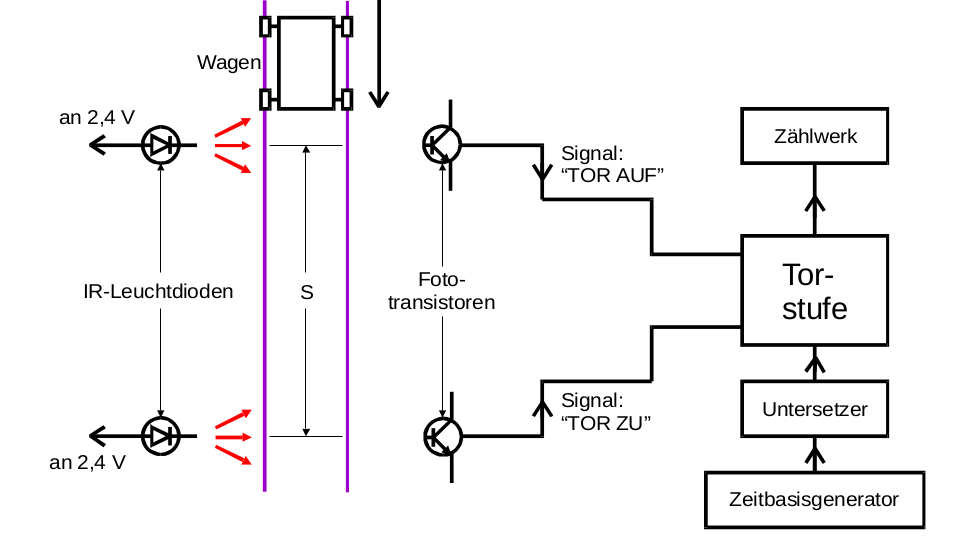
\includegraphics{Bilder/wagengeschwindigkeit.png}
	\caption{Prinzipieller Aufbau zur Untersuchung der Wagengeschwindigkeit. \cite{Anleitung}}
	\label{fig:wagen} %eventuell ersetzen mit den eigenen Schaltplänen, kann ich am we mal machen
\end{figure}
Zur Messung der Geschwindigkeit des Wagens wird die Schaltung wie in Abbildung \ref{fig:wagen} aufgebaut.
Die Geschwindigkeit des Wagens soll bestimmt werden auf der Wegstrecke zwischen den beiden Lichtschranken im Abstand $s$.
Die Distanz $s$ wird mit einem Maßband ausgemessen.
Zur Bestimmung der Geschwindigkeit ist eine präzise Messung der Fahrzeit des Wagens auf der Strecke $s$ nötig.
Daher wird beim Durchfahren der ersten Lichtschranke die Zeitmessung gestartet, und beim Durchfahren der zweiten Lichtschranke die Zeitmessung gestoppt werden.
Beim Durchfahren der ersten Lichtschranke sendet diese über eine Schmitt-Trigger einen kurzen \textbf{LOW}-Impuls. Dieser schaltet über den \textbf{\={S}}-Eingang einer bistabilen Kippstufe deren \textbf{Q}-Ausgang auf \textbf{HIGH}.
Vom \textbf{Q}-Ausgang wird das Signal an ein \textbf{AND}-Gatter geschaltet,
an dessem zweiten Eingang der Untersetzer mit dem Zeitbasisgenerator angeschlossen ist.
Solange an \textbf{Q} ein \textbf{HIGH}-Potential anliegt, gelangen also die durch den Zeitgeber erzeugten (und durch den Untersetzer faktorisierten) Schwingungen in das Zählwerk, welches die Schwingungen zählt.
Die Zeitmessung wird gestoppt, indem das \textbf{LOW}-Signal an der zweiten Lichtschranke  bei der Durchfahrt des Wagens auf den \textbf{\={R}}-Eingang der bistabilen Kippstufe gegeben wird,
sodass am Ausgang \textbf{Q} das Potential auf \textbf{LOW} geändert wird. Die Torstufe (realisiert als \textbf{AND}-Gatter) wird also geschlossen und die Schwingungen erreichen nicht mehr das Zählwerk.
Es werden für jeden Gang des Antriebsmotor des Wagens jeweils 5 Messungen für den Hin-und Rückweg durchgeführt.


\subsection{Messung der Frequenz der Schallwelle bei ruhendem Lautsprecher}
\label{sec:schall} %zu faul zum ändern
Die Messung der Frequenz der Schallwelle bei ruhendem Lautsprecher wird ermittelt mittels der in Abschnitt \ref{sec:frequenz} ausführlich erklärten Schaltung.
Diese wird hier allerdings manuell ausgelöst und dient lediglich dazu, dass die Schwingungen des Zeitbasisgenerators nur für eine fest definierte Zeit gezählt werden.
Diese fest definierte Zeit wird am Untersetzer zu $\SI{1}{\second}$ eingestellt. Am Zählwerk kann somit direkt die Frequenz $\nu_{\mathrm{0}}$ in $\si{\per\second}=\si{\Hz}$ abgelesen werden.
Die Messung wird zehnmal wiederholt.
\subsection{Messung der Schallgeschwindigkeit über die Wellenlänge}
Die Schallgeschwindigkeit bei Zimmertemperatur lässt sich bestimmen über die Kenntnis der Frequenz $\nu_{\mathrm{0}}$ des ruhenden Lautsprechers und der Wellenlänge $\lambda$ der Schallwelle.
Die Wellenlänge wird über \textbf{LISSAJOUS-Figuren} bestimmt.
Diese entstehen, wenn auf beide Achsen eines Oszilloskops Schwingungen aufgegeben werden. Dazu wird auf die X-Achse des Oszilloskops das verstärkte Ausgangssignal des Mikrophons und auf die Y-Achse das Signal des Sinusgenerators gegeben.
Jede Entartung der \textbf{LISSAJOUS-Figuren} zu einer Geraden stellt eine Phasenverschiebung von $\pi$ zwischen den beiden auf die Achsen gegebenen Schwingungen dar.
Mittels der Mikrometerschraube lässt sich, wie ersichtlich in Abbildung \ref{fig:lisa}, der Abstand zwischen Mikrophon und Lautsprecher variieren.
Für jede Entartung des Oszilloskopbilds zu einer Geraden wird anhand
der Maßskala an der Mikrometerschraube die Differenz zwischen zwei Entartungen bestimmt. Diese entspricht der halben Wellenlänge $\frac{\lambda}{2}$.
Mittels der bereits in Abschnitt \ref{sec:schall} bestimmten Frequenz der Schallwelle kann nun die Schallgeschwindigkeit bestimmt werden.

\begin{figure}
	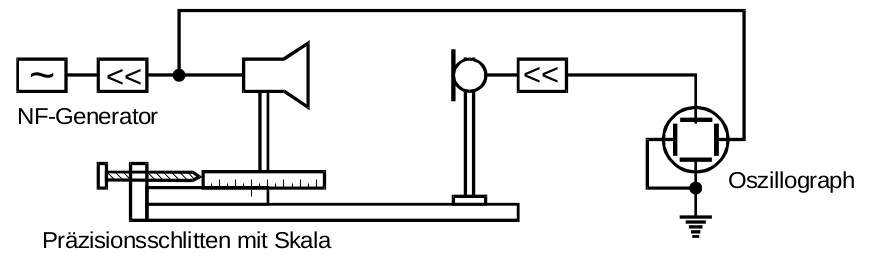
\includegraphics{Bilder/lissajou.png}
	\caption{Aufbau zur Messung der Schallgeschwindigkeit bei Raumtemperatur. \cite{Anleitung}}
	\label{fig:lisa}
\end{figure}


\subsection{Messung der Frequenz der Schallwelle bei bewegter Quelle}
\label{sec:frequenz}
In Abbildung \ref{fig:delphin} ist der prinzipielle Aufbau zur Bestimmung der Frequenz $\nu_{\mathrm{Q}}$ bei bewegter Quelle dargestellt.
Der Wagen mit dem Lautsprecher bewegt sich nun relativ zum Empfänger mit den in Abschnitt \ref{sec:speedygonzales} bestimmten Geschwindigkeiten.
Jede Messung wird erneut für jeden Gang des Antriebmotors jeweils fünfmal für den Hin-als auch den Rückweg durchgeführt.
Das Zählwerk zählt, wie in Abschnitt \ref{sec:schall} bereits beschrieben, genau eine Sekunde lang die Schwingungen der Schallquelle, welche am Empfänger eintreffen. Es wird also die Frequenz der Schallwelle, welche am Empfänger eintrifft, auf dem Zählwerk ausgegeben.
Um dies zu erreichen, wird das \textbf{LOW}-Signal, welches erzeugt wird beim Durchfahren des Wagens durch die erste Lichtschranke, auf den \textbf{\={S}}-Eingang einer bistabilen kippstufe gegeben, sodass deren \textbf{Q}-Ausgang auf \textbf{HIGH}-Potential gestellt wird.
Dieses \textbf{HIGH}-Signal wird genutzt, um zwei Torstufen zu öffnen.
Eine der beiden Torstufen verbindet hierbei den Empfänger mit dem Zählwerk.
Die am Mikrophon registrierte Sinusschwingung wird zunächst allerdings zunächst noch über einen Signalwandler in eine \textbf{TTL}-rechteckschwingung umgewandelt, bevor das Signal über dei Torstufe auf das Zählwerk gegeben wird.
Die zweite Torstufe dient in der vorliegenden Schaltung der Steuerung der Zeitmessung.
Auf dem zweiten Eingang der zweiten Torstufe wird das Signal des Zeitbasisgenerators aufgegeben.
Da der Ausgang der zweiten Torstufe (auch hier erneut realisiert über \textbf{AND}-Gatter) an den Untersetzer angeschlossen ist, muss dieser nun nur noch so eingestellt werden, dass dieser genau nach einer Sekunde ein Signal
zur weiteren Steuerung der Schaltung weitergibt.
Da der Zeitbasisgenerator jede Mikrosekunde einen Schwingungsimpuls, also $10^6$ Impulse pro Sekunde, muss der Untersetzer auf $10^6$ gestellt werden (Der Untersetzer zählt die Anzahl der eintreffenden Impulse, sobald der zuvor festgelegte Wert erreicht ist, sendet der Übersetzer ein \textbf{HIGH}-Impuls).
Das durch den Übersetzer gesendete \textbf{HIGH}-Signal wird auf den \textbf{T}-Eingang der bistabilen Kippstufe gegeben. Da die bistabile Kippstufe bei fallender Flanke (also \textbf{HIGH} zu \textbf{LOW}) am \textbf{T}-Eingang den Status am \textbf{Q}-Ausgang ändert, wird dieser auf \textbf{LOW} gesetzt und beide Torstufen der Schaltung deaktiviert.
Am Zählwerk kann die Frequenz $\nu_{\mathrm{Q}}$ jetzt direkt abgelesen werden.

\begin{figure}
	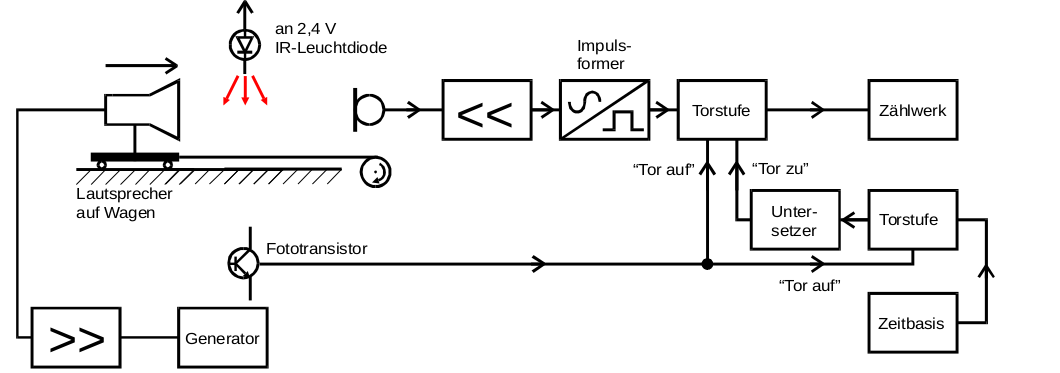
\includegraphics{Bilder/Frequenz.png}
	\caption{Aufbau zur Messung der Frequenz bei bewegter Quelle. \cite{Anleitung}}
	\label{fig:delphin}
\end{figure}

\subsection{Messung der Frequenz über die Schwebungsmethode}
Die Messung der Frequenz über die Schwebungsmethode erfolgt mit nahezu dem gleichen Aufbau wie im vorherigen Abschnitt.
Allerdings wird nun der Lautsprecher direkt neben dem Empfänger montiert.
Auf dem Wagen wird stattdessen ein Reflektor montiert. Dieser bewegt sich bezüglich des ruhenden Empfängers mit der Geschwindigkeit $2v$
Der Empfänger nimmt jetzt also sowohl die direkte Schallwelle des Lautsprechers, als auch die reflektierte Schallwelle auf.
Der Reflektor bewegt sich bezüglich des Empfängers. Dadurch entsteht aus der Überlagerung der direkt erzeugten und der reflektierten Schallwelle eine Schwbung.
Damit nur die Schwebung gemessen wird, muss vor den Signaleingang des Mikrophons im Aufbau \ref{fig:delphin} ein Tiefpass geschaltet werden.
Erneut werden für jeden Gang für Hin-und Rückweg jeweils fünf Werte aufgenommen.
